
\section{Predicting 2D joint candidate locations}

% Explain hourglass network, it's structure and why it's good.
The goal of the first stage is to take, for each video frame, an image reperesenting the animal and to output a $W \times H \times \njoints$ tensor of heatmaps. To achieve this, we train the stacked hourlgass network~\cite{newell2016stacked} of Newell et al. to a large dataset of synthetically generated quadruped images. 

\subsection{Generating synthetic quadruped images}

In order to render a synthetic quadruped image, a set of pose $\pose$, shape $\shape$ and position $\posn$ parameters are required. With these parameters, a (textureless) training image can be generated by applying \Cref{eq:render_sil} and corresponding ground truth 2D joints locations can be generated via \Cref{eq:project_joints}. What remains is to ensure a model trained on the synthetic images generalizes to the real-world test images. To achieve this, it is important that the training dataset captures the modes of variation by appropriately sampling the model parameters. 

\subsubsection{Sampling shape and pose parameters}

Given that the real-world test images exhibit multiple quadruped species, a primary mode of variation is the animal's \emph{shape} characterisitics. Naively, generating a dataset large enough to capture possible test animal shapes would be a challenging task, since it would require access to multiple real or artist-generated 3D scans. Fortunately, the SMAL model defines a linear shape space which allows repeated sampling of different (and realistic) quadruped shapes. Of course, having been built from only toy figurines, the variation is still somewhat limited, but as the later experimental section will show, the model is fit for purpose. Synthetic shape parameters $\shape$ are obtained by sampling from a Gaussian prior:

\begin{equation}\label{eq:sampling_shape}
X = Y
\end{equation}

Another mode of variation in test images is the various animal limb positions. These can again be synthetised by sampling from a gaussian prior constructed from a dataset of animal poses. Since no such dataset exists for real animals, a prior is instead built from a small set of artist-generated poses, originally provided by the SMAL model authors. The sampling strategy is therefore given by:


\begin{equation}\label{eq:sampling_pose}
    X = y
\end{equation}


\subsubsection{Sampling position (camera) parameters}

The random camera positions are generated as follows: the orientation of the camera relative to the animal is uniform in the range $[0, 2\pi]$, the distance from the animal is uniform in the range 1 to 20 meters and the camera height is in the range $[0,\frac{\pi}{2}]$. This smaller range is chosen to restrict unusual camera elevation. Finally, the camera ``look" vector is towards a point uniformly in a 1m cube around the animal's center, and the ``up" vector is Gaussian around the model Y axis.

\subsubsection{What about textures and backgrounds?} 

At this point, the synthetic test images have plausible shape, pose and positional parameters but are lacking in realistic texture. Furthermore, it is not clear how to render plausible background scenes, nor how to convincingly place the 3D animal in such a scene. This challenge allows for a primary contribution of this work: using the silhouette domain as a representation much easier to synthetise (since surface texture maps and background textures are lost) and can be obtained from real-world test images. Another important characteristic of the mapping between real-world images and silhouette counterparts is that the shape and pose information is mostly preserved, apart from a few ambiguities (e.g. limb ordering due to lacking interior contours). 

To summarise, training data comprises $(S, \kappa)$ pairs, that is pairs of binary silhouette images, and the corresponding 2D joint locations as a $2\times J$ matrix. See an example in   To generate each image, a random shape vector $\shape$, pose parameters $\pose$ and camera position $\posn$ are drawn, and used to render a silhouette $R\bigl(\posn * \verts(\pose, \shape)\bigr)$ and 2D joint locations $\kappa(\posn,\pose,\shape)$.


% The corresponding 2D joint positions, represented as a $2\times \njoints$ matrix are given, as above, by
% \[
%     \kappa(\posn, \pose, \shape) := \proj(\posn * \verts(\pose, \shape) \jointselect)
% \]

\subsection{Prediction of 2D joint locations using multimodal heatmaps}

% explain that the quality of the joint prediction, while good still leaves unsatisfactory predictions which can cause problems to the later energy minimization steps. To overcome this, 


A pose estimation network can now be trained on a dataset of binary silhouette images $S$ with corresponding 2D joint locations $\kappa(\posn,\pose,\shape)$. The core network architecture used for this task is the stacked hourglass network~\cite{newell2016stacked} of Newell et al., with an adaptation to produce multi-modal outputs. The stacked hourglass network is now briefly described:

\subsubsection{Stacked hourglass network}

A stacked hourglass network is a convolutional neural network specifically designed for the task of pose estimation. Hourglass allows inference to take place across multiple scales; an important advantage allowing the network to reason about global information (such as the full body) and local information (such as face features). This is achieved using a repeated bottom-up, top-down modules which each produce a $W \times H \times \njoints$ heatmap tensor. Supervision is applied to each of these heatmaps, which are then passed to ths subsequent block, allowing high level features to be reevaluated for higher order spatial relationships (generally only present at low resolutions). The network's architecture can be seen in detail in Figure XXX. Hourglass uses a mean squared error loss against a ground truth heatmap tensor, which is applied to the network's final output and all intermediatary hetamaps. Therefore, ground truth joint coordinates $\kappa(\posn,\pose,\shape)$ must first be encoded into a $W \times H \times \njoints$ tensor of heatmaps. The original authors find that the network has better convergence properties if the ground truth heatmaps are blurred slightly, since a gradient is then provided to predicted ``near misses''. This is achieved by blurring ground truth heatmaps with a Gaussian kernel of radius $\sigma$. The final 2D joint positions are then obtained using non-maximum suppression on the output heatmaps

\begin{equation}\label{eq:non-max-suppression}
    A = B    
\end{equation}

\subsubsection{Adaptations for training on synthetic data}

This setup is mostly suitable for training on synthetic quadruped data, subject to a couple of adaptations. Firstly, the silhouette training images differ considerably in appearance to the RGB images used by the original Hourglass authors. A common difficulty for training pose estimation networks on full RGB images is in trying to distinguish between objects and the background class. With binary silhouette images, this distinction is made trivial as background and foreground are assigned values $0$ or $1$ respectively. Unfortunately, this causes a problem when naively training HourglassNet on the generated synthetic images as the network can greatly minimize the loss by simply predicting `background' for every image pixel (since background pixels tend to outnumber foreground pixels). The fact that `background' is a much simpler class to predict than the other joint classes causes a training instability which is challenging to overcome by adjusting the learning rate. Instead, the loss function is replaced with a \emph{weighted} version of the mean squared error loss. This modification encourages the network to devote it's attention to all classes equally. The precise formulation for this is given as follows:

\begin{equation}\label{eq:weighted-mse}
    A = B
\end{equation}


\subsubsection{Adapting stacked hourglass network for multi-output learning}

As detailed in the later experimental section, the network trained using this process generalizes well from synthetic to real images due to the use of the silhouette, and produces accurate predictions for most joints. However, the predictor performs poorly on some joints due to ambiguities which result from the lack of interior contours in the silhouette input data. These missing details cause often result in confusion between joint ``aliases'': left and right or front and back legs.  When these predictions are wrong and are represented by high confidence heatmap regions, little probability mass is assigned to the area around the correct leg, meaning no available proposal is present after non-maximal suppression.

This is handled with a further technical contribution; handling the prediction uncertainty by adapting the stacked hourglass network to produce multiple outputs. This is achieved by explicitly training the network to assign some probability mass to the ``aliased'' joints. For each joint, a list of potential aliases are defined as weights $\lambda_{j,j'}$ and linearly blend the unimodal heatmaps $G$ to give the final training heatmap $H$:

\begin{equation}
    H_{j}(p) = \sum_{j'} \lambda_{j,j'} G(p; \kappa_{j'}, \sigma)
\end{equation}

For non-aliased joints $j$ (all but the legs), $\lambda_{j,j} = 1$ and $\lambda_{j,j'} = 0$, yielding the unimodal maps. For aliased joints, the joint is assigned a weight $\lambda_{j,j} = 0.75$ and aliases are assigned a weight $\lambda_{j,j'} = 0.25$. This ratio is shown to ensure opposite legs have sufficient probability mass to pass through a modest non-maximal suppression threshold without overly biasing the skeleton with maximal predicted confidence. An example of a heatmap predicted by a network trained on multimodal training samples is illustrated in \figref{single_multi}. Note that the construction of at most bi-modal ground truth heatmaps sets a practical constraint on the number of output modes. In other words, the loss is minimized if the network produces one output mode for non-aliased joints and two output modes for aliased joints. 

% % Please add the following required packages to your document preamble:
% \usepackage{booktabs}
\begin{table}[]
    \begin{tabular}{@{}lllll@{}}
    \toprule
    Joint ID & Joint Name                    & Weight & Alias                         & Alias Weight \\ \midrule
    0        & Left front leg: paw           & 0.75   & Right front leg: paw          & 0.25         \\
    1        & Left front leg: middle joint  & 0.75   & Right front leg: middle joint & 0.25         \\
    2        & Left front leg: top           & 0.75   & Right front leg: top          & 0.25         \\
    3        & Left rear leg: paw            & 0.75   & Right rear leg: paw           & 0.25         \\
    4        & Left rear leg: middle joint   & 0.75   & Right rear leg: middle joint  & 0.25         \\
    5        & Left rear leg: top            & 0.75   & Right rear leg: top           & 0.25         \\
    6        & Right front leg: paw          & 0.75   & Left front leg: paw           & 0.25         \\
    7        & Right front leg: middle joint & 0.75   & Left front leg: middle joint  & 0.25         \\
    8        & Right front leg: top          & 0.75   & Left front leg: top           & 0.25         \\
    9        & Right rear leg: paw           & 0.75   & Left rear leg: paw            & 0.25         \\
    10       & Right rear leg: middle joint  & 0.75   & Left rear leg: middle joint   & 0.25         \\
    11       & Right rear leg: top           & 0.75   & Left rear leg: top            & 0.25         \\
    12       & Tail start                    & 1.0    &                               &              \\
    13       & Tail end                      & 1.0    &                               &              \\
    14       & Base of left ear              & 1.0    &                               &              \\
    15       & Base of right ear             & 1.0    &                               &              \\
    16       & Nose                          & 1.0    &                               &              \\
    17       & Chin                          & 1.0    &                               &             
    \end{tabular}
\end{table}\label{tab:joint_weights}

\begin{figure}[t]
% \begin{floatrow}
% \ffigbox{%%%%%%%%%%%%
\centering
\begin{tabular}{cc}
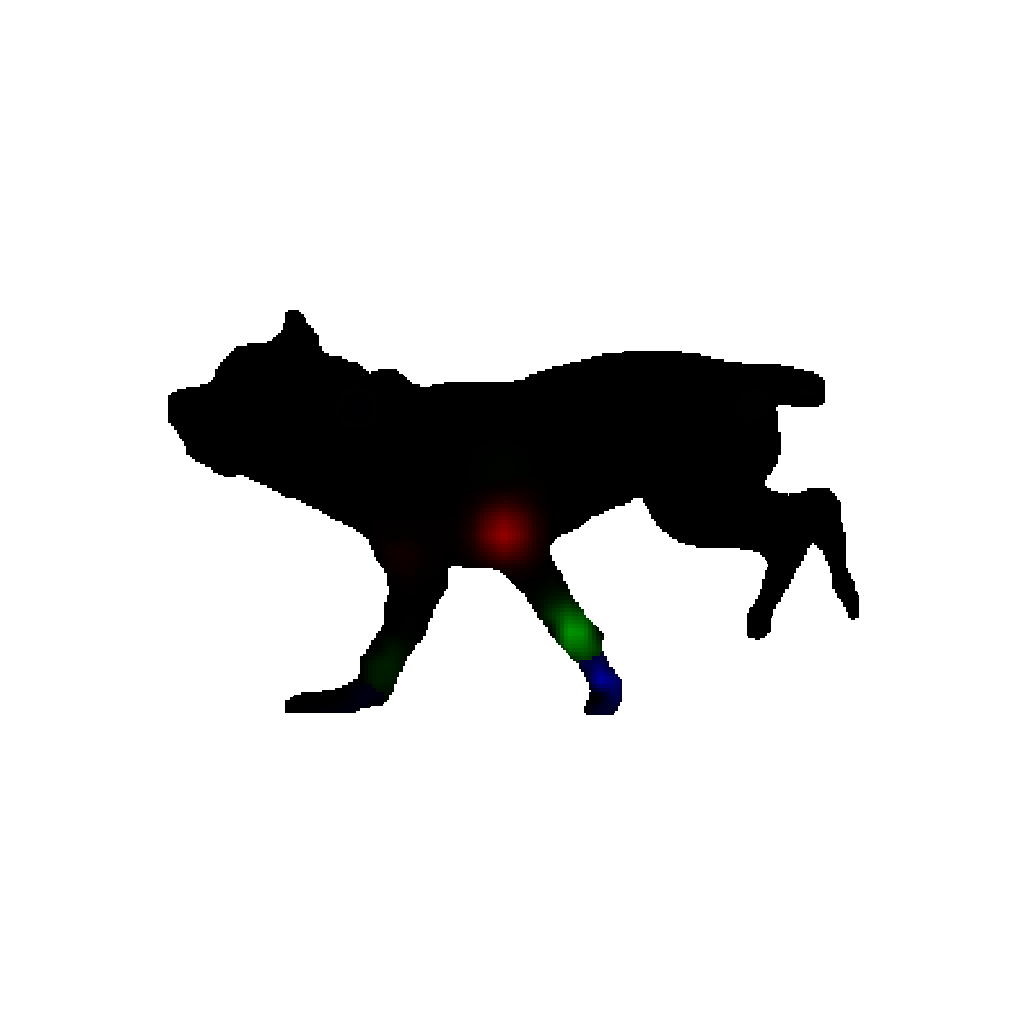
\includegraphics[trim={4cm 10cm 4cm 10cm},clip,width=0.5\linewidth]{single_vs_multi_new/left_heatmap_single.png} &
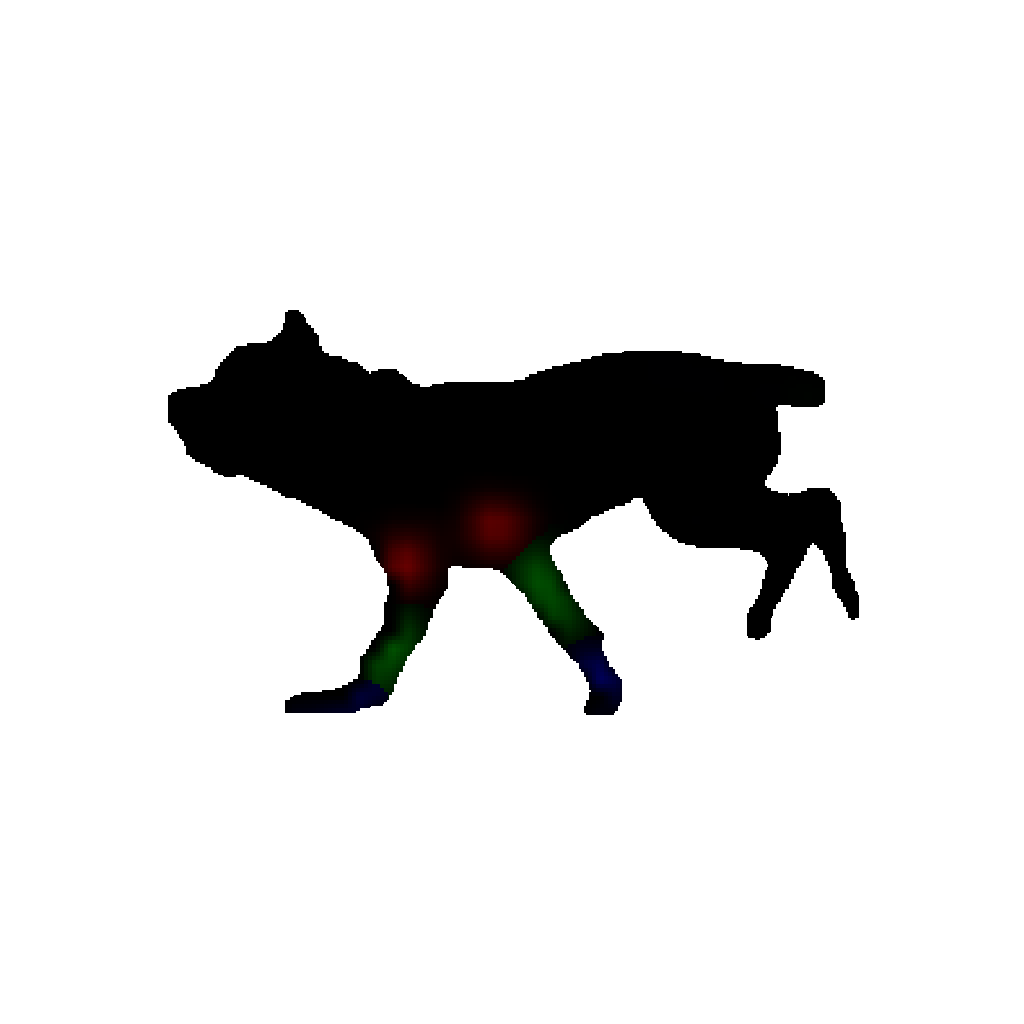
\includegraphics[trim={4cm 10cm 4cm 10cm},clip,width=0.5\linewidth]{single_vs_multi_new/left_heatmap_multi.png} \\
\end{tabular}
% }
{
\caption{Example predictions from a network trained on unimodal (top) and multi-modal (bottom) ground-truth  for front-left leg joints.}
\label{fig:single_multi}
}
% \end{floatrow}
\end{figure}

\begin{figure}[t]
% \begin{floatrow}
% \ffigbox{
\centering
\def\lp#1#2{\labelledpic{\includegraphics[width=0.20\linewidth]{#2}}{#1}}
\begin{tabular}{cccc}
\lp a{skeletons_new/skeleton_rgb_dog_cropped.jpg}&
\lp b{skeletons_new/skeleton_rgb_impala_cropped.jpg}&
\lp c{skeletons_new/skeleton_rgb_rhino_cropped.jpg}&
\lp d{skeletons_new/skeleton_rgb_horsejump-high_cropped.jpg}\\
\end{tabular}
% }
{
\caption{Example outputs from the joint prediction network, with maximum likelihood predictions linked into skeleton.}
\label{fig:exp-network}
}
% \end{floatrow}
\end{figure}